\chapter{Implementación y Prueba}\label{cap:implementacion-test}

\section{Introducción}
Este capítulo se centra en la implementación y validación del componente desarrollado. Se presentan los resultados más relevantes derivados de las pruebas realizadas, garantizando así el correcto funcionamiento del sistema y su conformidad con los requisitos establecidos por el cliente.



\section{Etapa de Implementación}

\subsection{Stack Tecnológico Seleccionado}
La elección del stack tecnológico se fundamentó en la perspectiva de mantener y continuar el desarrollo de la plataforma a largo plazo. Considerando que el laboratorio IALAB ofrece cursos de Python, Javascript y React, se optó por utilizar estos lenguajes, anticipando que los graduados de dichos cursos podrían constituir una valiosa fuente de recursos para posiciones de becarios en el proyecto.

Además de Python, Javascript y React, se seleccionaron otras tecnologías clave para la implementación de la plataforma. Para la base de datos, se eligió PostgreSQL, un sistema de gestión de bases de datos relacional robusto y de código abierto. En cuanto al componente de almacenamiento en memoria y coordinación de comunicaciones en tiempo real, se incorporó Redis. Para el desarrollo de la API REST, se adoptó Django Rest Framework (DRF), una potente herramienta que facilita la creación de servicios web con Django.


\subsection{Diagrama de Paquetes en el Backend}

En el diagrama de paquetes del backend (Figura \ref{fig:backend-packages}), se presenta una estructura clara y organizada del sistema implementado con Django. El directorio principal, denominado \textit{api patrocinio}, se destaca en azul y alberga la definición de todas las URL y la configuración global del proyecto.

En color amarillo, se identifican los módulos de la API REST, encapsulando las diferentes funcionalidades de la aplicación. En verde, se encuentran los archivos de plantillas y recursos que contribuyen a la presentación de la interfaz y el envío de emails.

\begin{figure}[H]
\centering
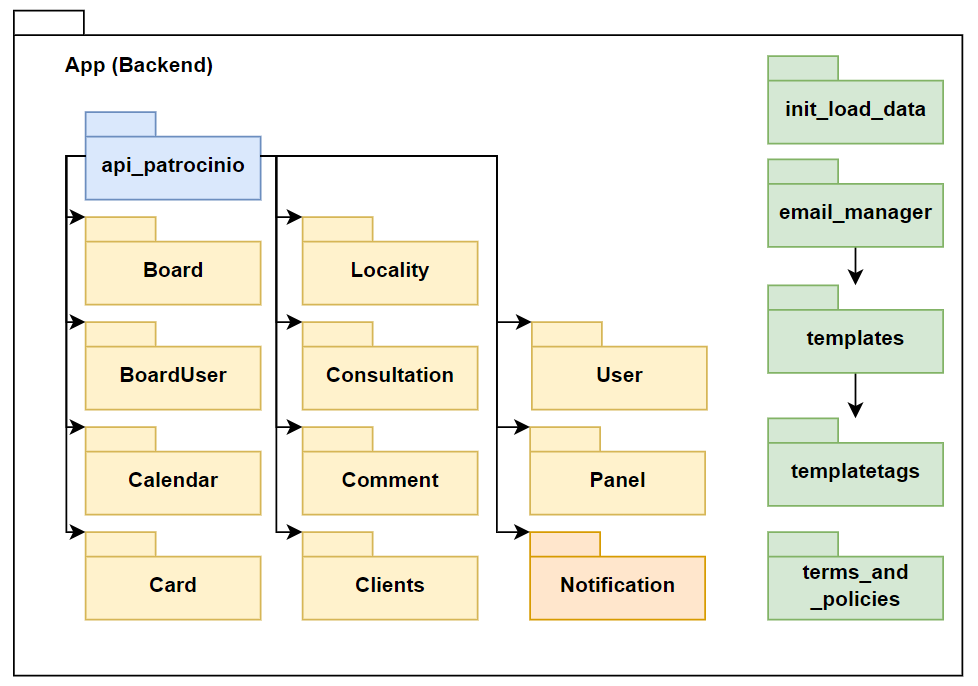
\includegraphics[width=0.80\linewidth]{fig/paquete-backend.png}
\caption{Diagrama de Paquetes del Backend}
\label{fig:backend-packages}
\end{figure}

\subsection{Diagrama de Paquetes en el Frontend}

En el diagrama de paquetes del frontend (Figura \ref{fig:frontend-packages}), se observa la estructura organizada de la interfaz de usuario desarrollada en React. El directorio \textit{pages}, en amarillo, contiene las definiciones de las páginas, que a su vez alojan contenedores, pudiendo contener otros contenedores y/o componentes.

\begin{figure}[H]
\centering
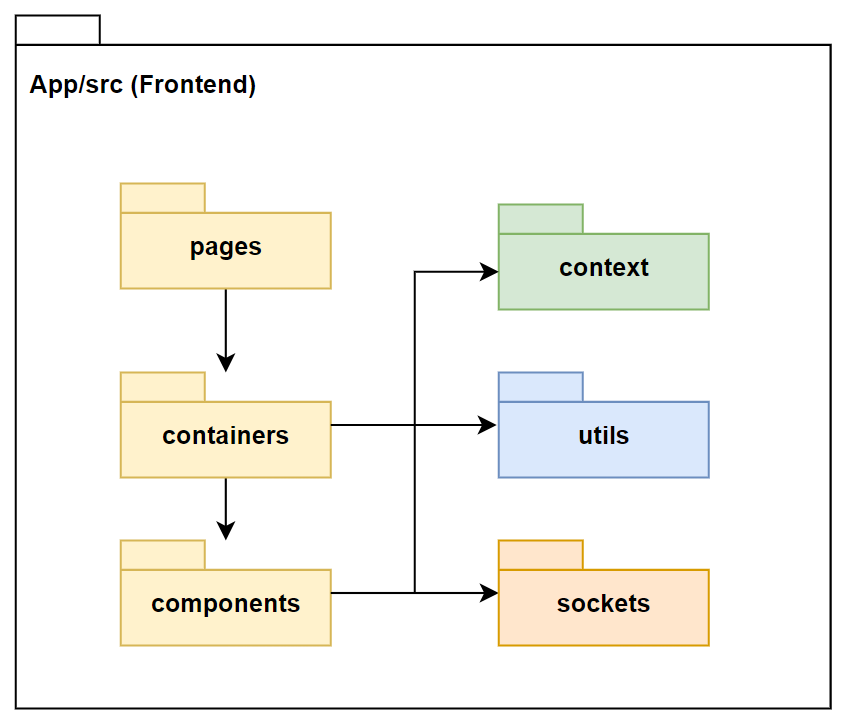
\includegraphics[width=0.65\linewidth]{fig/paquete-frontend.png}
\caption{Diagrama de Paquetes del Frontend}
\label{fig:frontend-packages}
\end{figure}

El directorio \textit{pages} encapsula definiciones simples de cada página, gracias a la reutilización de código proporcionada por los contenedores y componentes. Dentro del directorio \textit{containers}, se encuentran los contenedores que agrupan un conjunto de componentes destinados a una interfaz o funcionalidad específica. Por otro lado, el directorio \textit{components} contiene las definiciones de los componentes individuales.

En verde, el directorio \textit{context} almacena los proveedores utilizados en el proyecto React, como el proveedor de información del usuario. Este enfoque permite gestionar eficientemente el estado de la aplicación y compartir información relevante entre componentes.

La lógica para el procesamiento y la obtención de datos desde el backend se encuentra en el directorio \textit{utils}, resaltado en azul. Este directorio actúa como un repositorio centralizado para las funciones y utilidades esenciales utilizadas en todo el proyecto, promoviendo la coherencia y el mantenimiento eficiente del código.

Finalmente, en naranja, el directorio \textit{sockets} contiene los consumidores del sistema de notificaciones en tiempo real, lo que contribuye significativamente a la implementación de esta funcionalidad clave. La capacidad de actualización dinámica de las vistas por eventos y el envío de alertas se logra mediante estos consumidores, mejorando la experiencia del usuario al mantenerlo informado en tiempo real sobre eventos relevantes.



\subsection{Integración con Google Forms}\label{subsec:integracion-google-form}

La integración con Google Forms se ha llevado a cabo mediante el desarrollo de plugins que optimizan la recolección y organización de datos a través de formularios. A continuación, se detallan los aspectos clave de esta integración:

\subsubsection{Características de Google Forms:}
Google Forms se presenta como una herramienta versátil y gratuita para la recopilación de datos a través de formularios. Su facilidad de uso y la familiaridad que tienen los usuarios con esta plataforma, gracias a su implementación en el ámbito del patrocinio jurídico de la UBA, fueron determinantes en su elección. Además, los formularios de Google pueden integrarse en correos electrónicos y páginas web, ampliando su versatilidad.

\subsubsection{Desafíos y Soluciones en la Estructuración de Preguntas:}
Uno de los desafíos encontrados fue la limitación en la diversidad de tipos de datos disponibles en los formularios. Esto se volvió problemático cuando un conjunto de preguntas dependía de otra, como en el caso de la selección de la nacionalidad, provincia y localidad. La solución adoptada fue conceptualizar cada grupo como una sección independiente, facilitando la navegación del usuario a través de las diferentes opciones.

Dada la complejidad del proceso, la cantidad de volumen inusable proporcionado a la base de datos si se tenían en cuenta todas las localidades del mundo,  se decidió restringir a provincias y localidades de Argentina. Para países extranjeros, se permite recuperar únicamente la nacionalidad, registrando la provincia y la localidad como campos de texto en Google Forms. Aunque estos últimos no son recolectados por el sistema para garantizar la compatibilidad con la base de datos, pueden ser ingresados manualmente por un administrador si es necesario.

\subsubsection{Automatización de la Carga de Preguntas:}
La carga manual de datos para las localidades, provincias y nacionalidades se optimizó mediante una hoja de cálculo con opciones de filtro por nacionalidad y un script generado en Google Apps Script \ref{sec:mt:app-script}. Estos recursos, están disponibles en el repositorio de la unidad (ver \ref{sec:repo-git}), adicionalmente se deberá establecer vínculos manuales entre preguntas para redirigir a los usuarios a las secciones correspondientes según sus elecciones.

\subsubsection{Manejo de Formularios Específicos:}
Para casos específicos, como el registro de hijos de un consultante, se creó un formulario separado debido a las limitaciones de Google Forms en la gestión dinámica de la cantidad de hijos que un consultante podría tener. Además, se diseñó un formulario exclusivo para consultas, vinculando la consulta con el consultante mediante su documento de identidad (DNI o pasaporte).

\subsubsection{Envío de Datos al Sistema Case Management System:}

Para el envío de la información recopilada a través de los formularios, se implementaron endpoints dedicados para cada tipo de formulario en la API REST. Además, se diseñaron funciones en Google Apps Script que se ejecutan al enviar un formulario, encargadas de recuperar y transformar los datos antes de transmitirlos a la API REST del proyecto. En caso de fallos en este proceso, el sistema notificará a través de correo electrónico sobre la imposibilidad de enviar los datos, asegurando una comunicación eficiente en caso de inconvenientes.

Para obtener información adicional sobre las interfaces, consulte la sección de anexos \ref{cap:anexo-expoint-forms}.


La implementación de estas funcionalidades se puede encontrar en el directorio \href{https://github.com/proyecto-patrocinio/proyecto-patrocinio/tree/main/com/script-forms}{proyecto-patrocinio/com/script-forms/} del repositorio del proyecto. Para incorporar estos archivos al formulario correspondiente, simplemente abra el editor del formulario, seleccione los tres puntos, vaya a ``Editor de secuencias de comandos'' y agregue los archivos correspondientes.


La Figura \ref{fig:app-script-code} muestra una captura de pantalla del código en Google Apps Script.

\begin{figure}[H]
\centering
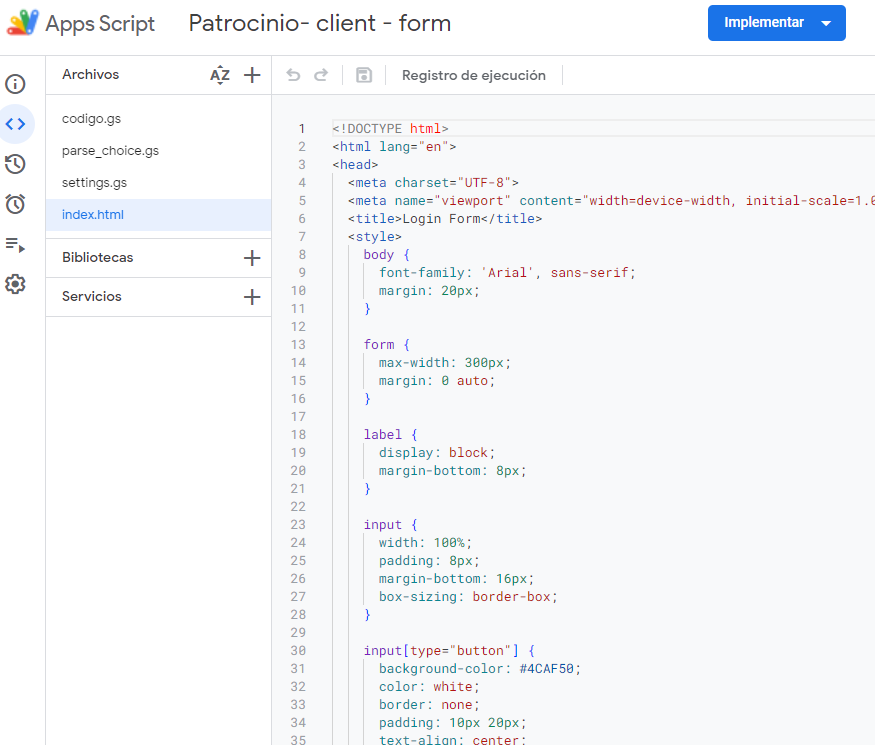
\includegraphics[width=0.75\linewidth]{fig/app-script-code.png}
\caption{Captura de pantalla del código en Google Apps Script.}
\label{fig:app-script-code}
\end{figure}

Adicionalmente, se deben configurar los activadores (ver Figura \ref{fig:activadores} y \ref{fig:activador-api-send-form}) siguiendo las instrucciones del README del repositorio. Por ejemplo, en el formulario ``Clients'', se necesitan los activadores: ``onFormOpen'' (explicado en la sección \ref{subsubsec:app-script-menu}), ``updateCredentials'' (explicado en la sección \ref{subsubsec:refresh-token}) y ``onFormSubmit''.

\begin{figure}[H]
\centering
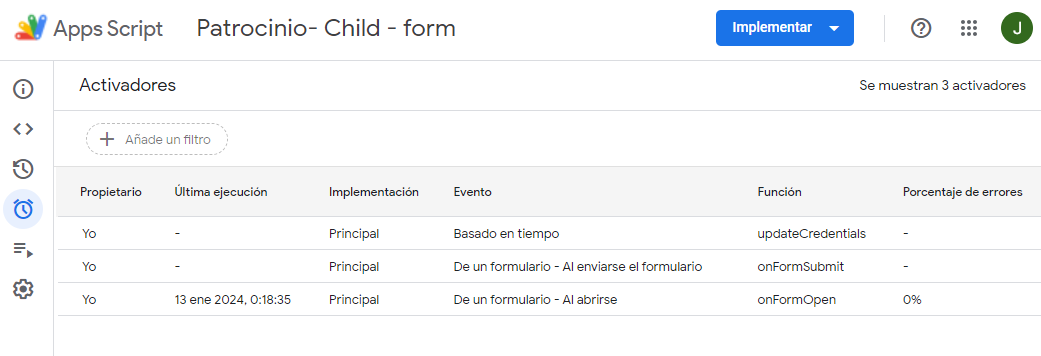
\includegraphics[width=0.90\linewidth]{fig/activadores.png}
\caption{Configuración de activadores.}
\label{fig:activadores}
\end{figure}

El activador ``onFormSubmit'' debe agregarse a los tres formularios y se encargará de ejecutar las funciones para el envío del formulario a la API.

\begin{figure}[H]
\centering
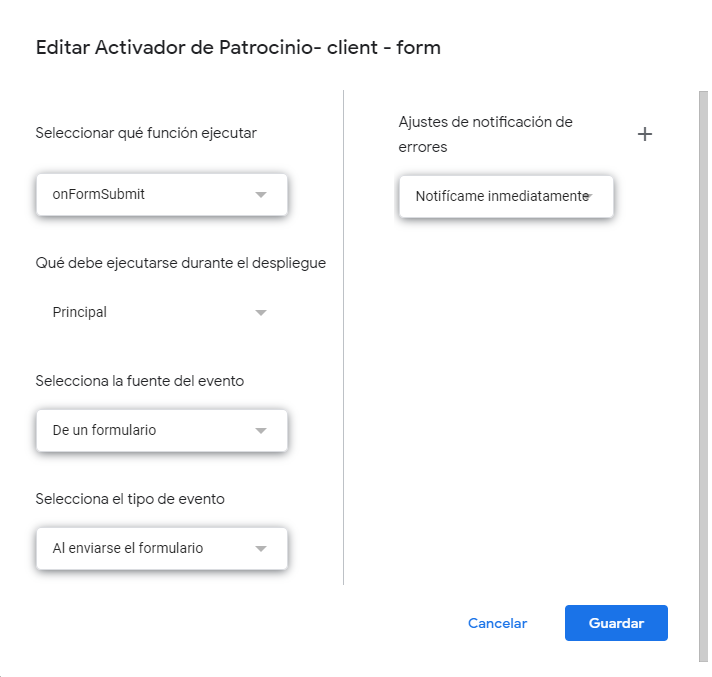
\includegraphics[width=0.75\linewidth]{fig/activador-api-send-form.png}
\caption{Activador para el envío del formulario a la API.}
\label{fig:activador-api-send-form}
\end{figure}





\subsubsection{Seguridad y Autenticación:}\label{subsubsec:app-script-menu}
Se estableció un rol especial para Google Forms con el fin de garantizar la conexión segura con el sistema. Se requiere proporcionar las credenciales de un usuario con este rol en cada formulario. Para facilitar la gestión de estas credenciales, se implementó un plugin de menú mediante Google Apps Script, ofreciendo opciones para cargar credenciales y refrescar tokens de forma intuitiva.

La implementación de esta funcionalidad implica agregar los archivos del directorio \href{https://github.com/proyecto-patrocinio/proyecto-patrocinio/tree/main/com/script-forms/common}{proyecto-patrocinio/com/script-forms/common} del repositorio en los tres formularios.

En la Figura \ref{fig:forms-menu-1}, se muestra la ubicación del plugin del menú en la esquina superior derecha del formulario.

\begin{figure}[H]
    \centering
    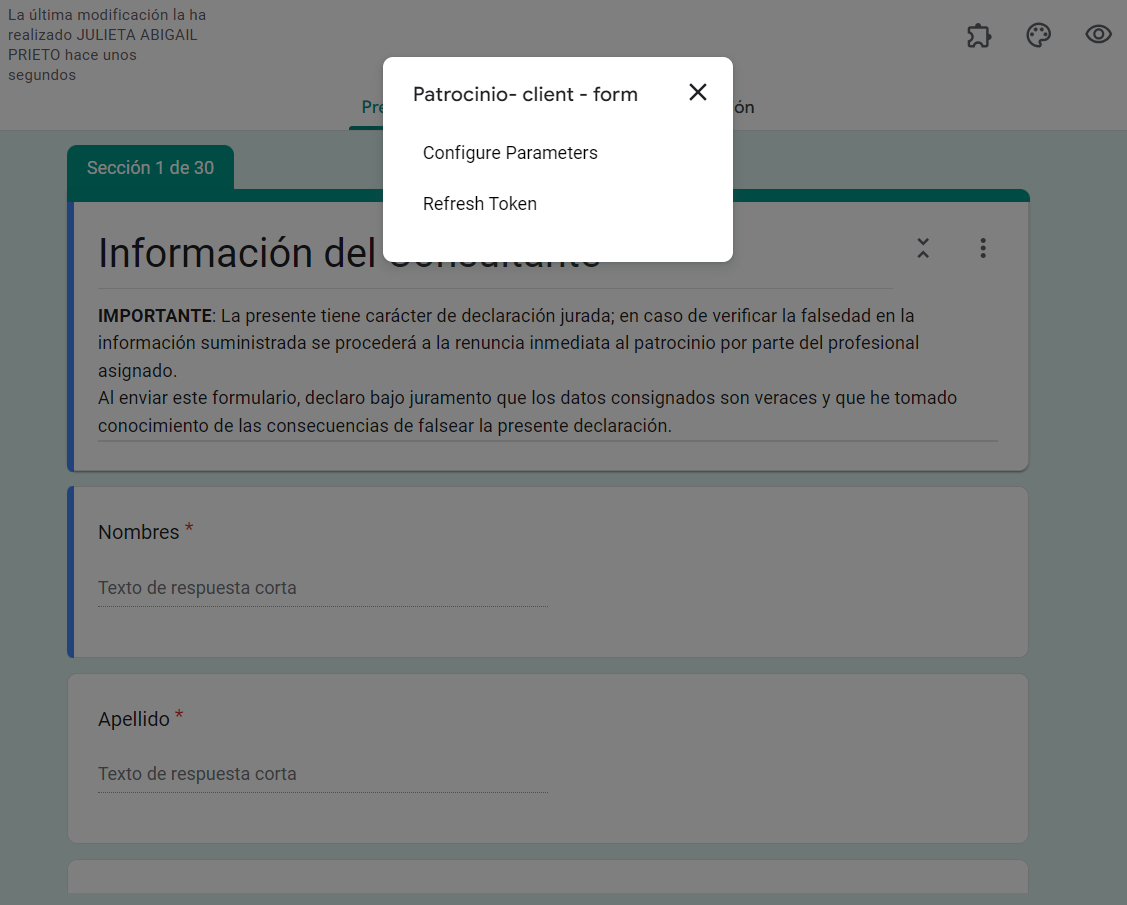
\includegraphics[width=1\linewidth]{fig/forms-menu-2.png}
    \caption{Ubicación del Plugin de Menú en Google Forms}
    \label{fig:forms-menu-1}
\end{figure}

En la Figura \ref{fig:froms-menu-parameters}, se presenta la interfaz de configuración del plugin. Aquí, se debe establecer, por única vez, el nombre de usuario y la contraseña del usuario de Case Managment System con permisos específicos para ``forms'', la URL para iniciar sesión, es decir \textbf{https://\{\{domain\}\}/api/auth/login/}, y la URL del endpoint correspondiente, como por ejemplo \textbf{https://\{\{domain\}\}/api/consultations/consultation/form/} para el formulario de consultantes.

\begin{figure}[H]
    \centering
    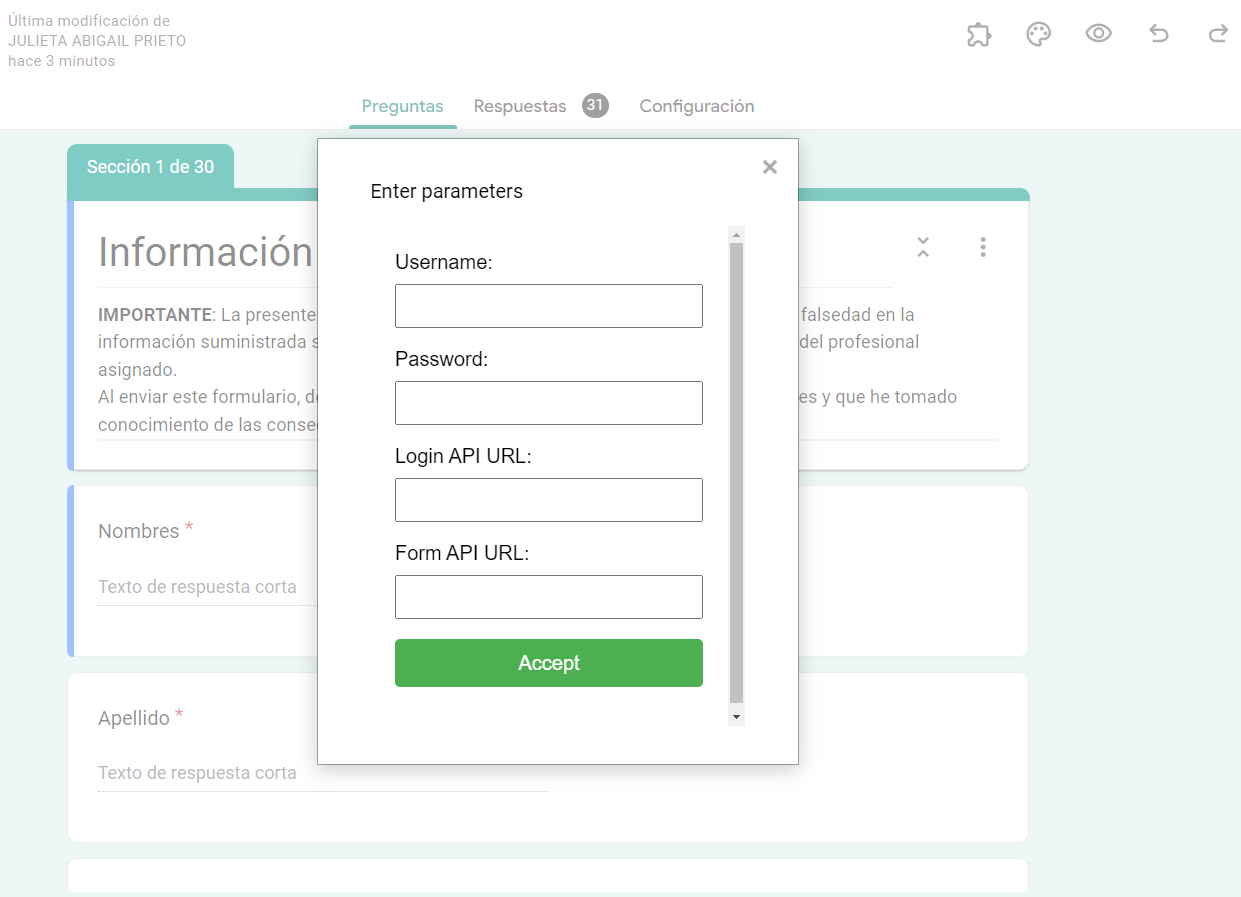
\includegraphics[width=1\linewidth]{fig/forms-menu-parametros.png}
    \caption{Interfaz de Configuración del Plugin de Menú}
    \label{fig:froms-menu-parameters}
\end{figure}

Para obtener información detallada, consulte el README y los archivos de notas en cada directorio correspondiente al formulario en el repositorio.

\subsubsection{Refresco Automático de Tokens:}\label{subsubsec:refresh-token}

Con el objetivo de mejorar la eficiencia del sistema, se ha implementado un activador que ejecuta automáticamente el proceso de refresco del token en intervalos regulares. Aunque es posible realizar este proceso manualmente, se recomienda configurar la opción automática para garantizar la continuidad segura de la conexión.

Para implementar esta funcionalidad, además de agregar los archivos del directorio \href{https://github.com/proyecto-patrocinio/proyecto-patrocinio/tree/main/com/script-forms/common}{proyecto-patrocinio/com/script-forms/common} en el repositorio, es necesario crear manualmente el activador. Se sugiere configurar el activador para que ejecute el refresco del token diariamente, preferiblemente durante un horario nocturno.

En la Figura \ref{fig:activador-credentials-form}, se muestra cómo crear el activador de forma manual.

\begin{figure}[H]
    \centering
    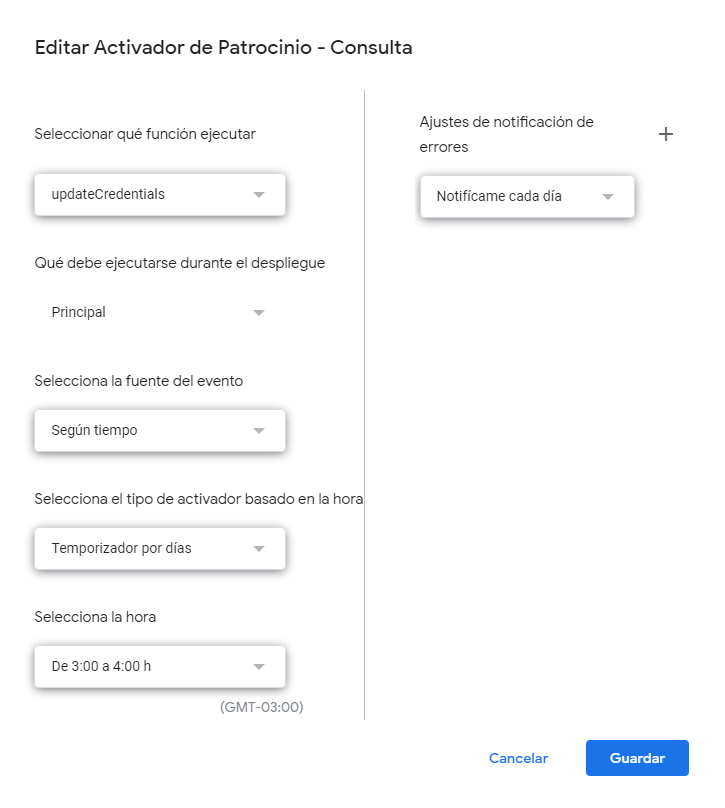
\includegraphics[width=1\linewidth]{fig/activador-credentials-form.png}
    \caption{Activador para el Refresco Automático del Token}
    \label{fig:activador-credentials-form}
\end{figure}



\subsection{Nginx como Servidor y Reverse Proxy}
En la infraestructura de la plataforma, se utiliza Nginx como reverse proxy para dirigir el tráfico a los diferentes servicios. La estructura general se compone de tres servicios principales: el frontend con Node, la API REST de Django alojada en Gunicorn, y el sistema de notificaciones en tiempo real alojado en Dhapne.

Puede encontrar un template del archivo Nginx en el repositorio de deploy referenciado en la sección \ref{sec:repo-git}.

Adicionalmente, se ha añadido un archivo de configuración adicional de Nginx en el servidor para integrar el nuevo servicio en el sistema. Ambos archivos de configuración se encuentran detallados en el anexo, específicamente en el Apéndice \ref{cap:apendix-nginx}.

\subsubsection{Limitación de Solicitudes y Conexiones}

Se han implementado límites de solicitudes y conexiones utilizando las directivas \texttt{limit\_req\_zone} y \texttt{limit\_conn\_zone} de NGINX. Estas medidas ayudan a mitigar posibles ataques DDoS y garantizan un rendimiento óptimo del sistema al controlar la velocidad de las solicitudes y conexiones desde una sola dirección IP.

\subsubsection{Configuración de Redirecciones}

NGINX se encarga de redirigir las solicitudes a los servicios correspondientes mediante la configuración de las ubicaciones (\texttt{location}). Se han definido ubicaciones específicas para el frontend, la API REST y las conexiones WebSocket, asegurando un enrutamiento adecuado de acuerdo con los requisitos del sistema.

\subsubsection{Alias para Recursos Estáticos}

Se utiliza la directiva \texttt{alias} para configurar NGINX y servir recursos estáticos desde una ubicación específica, facilitando la gestión de archivos estáticos generados por Django para la interfaz de administración.

\subsubsection{Consideraciones Adicionales}

 El archivo de configuración en el servidor está configurado para manejar solicitudes HTTPS en el puerto 443 utilizando certificados SSL proporcionados por Certbot. Proporciona una capa adicional de seguridad al cifrar la comunicación entre el cliente y el servidor.

\subsection{Integración Continua}
Para asegurar la calidad del código y facilitar la entrega continua, se implementó un sistema de integración continua utilizando GitHub Actions (ver \ref{sec:mt:ci-cd}). Este sistema automatiza la verificación del código, la ejecución de pruebas y la generación de imágenes de Docker. Se establecieron dos pipelines independientes para el frontend y el backend de la aplicación.

Ambos pipelines se inician en respuesta a eventos específicos, el push a las ramas \texttt{main} y \texttt{dev}, la creación de nuevos \texttt{tags}, o la publicación de releases. A continuación, se describen las fases clave del pipeline:

\begin{itemize}
    \item \texttt{CI}: Se encarga de realizar verificaciones de salud en el código, ejecutar pruebas y garantizar el formato adecuado del mismo.
    \item \texttt{CD}: Se encarga de buildear y publicar las imágenes de Docker en Docker Hub.
\end{itemize}

\begin{figure}[H]
\centering
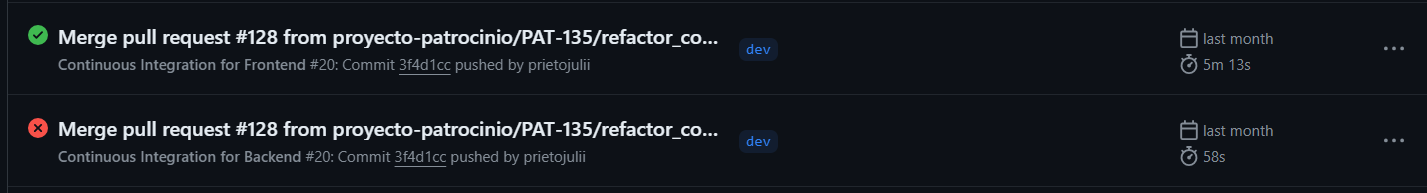
\includegraphics[width=1\linewidth]{fig/workflows.png}
\caption{Implementación de Pipelines en Github Actions}
\label{fig:workflows-implementacion}
\end{figure}

En la figura \ref{fig:workflows-implementacion}, se observa cómo el pipeline del frontend se activó correctamente tras la fusión de la rama PAT-135 en la rama dev, mientras que el pipeline de la rama backend experimentó un fallo. Este enfoque resulta práctico e intuitivo, ya que GitHub proporciona una interfaz visual que permite verificar fácilmente el estado de los pipelines y revisar los registros en caso de errores.

\subsubsection{Política de Contraseñas Seguras}

Para fortalecer la seguridad de la plataforma, se ha establecido una política rigurosa con respecto a las contraseñas de los usuarios. Con el objetivo de proteger adecuadamente las cuentas, se requiere que las contraseñas cumplan con los siguientes criterios mínimos:

\begin{itemize}
    \item Longitud mínima de 8 caracteres.
    \item Inclusión de letras minúsculas y mayúsculas.
    \item Uso de al menos un número.
    \item Inclusión de al menos un carácter especial.
\end{itemize}

Esta política se implementa durante la creación y modificación de contraseñas, asegurando que los usuarios establezcan credenciales robustas que contribuyan a la protección de los datos. La exigencia de contraseñas seguras mitiga posibles riesgos de seguridad y garantiza un entorno confiable para todos los usuarios de la plataforma.

Además de manera predeterminada, Django emplea el algoritmo \textbf{PBKDF2} con un hash \textbf{SHA256}, un estándar de extensión de contraseña recomendado por el \textbf{Instituto Nacional de Estándares y Tecnología (NIST)}. Esta elección proporciona un alto nivel de seguridad y resiste eficazmente los intentos de descifrado, ya que requiere considerables recursos computacionales para ser comprometido. Por lo tanto las contraseñas se almacenan de forma segura en la base de datos.

\subsubsection{Autenticación Reforzada y Activación de Usuarios}

Con el propósito de elevar aún más los estándares de seguridad, se implementaron medidas adicionales en el proceso de creación y acceso de usuarios:

\begin{itemize}
    \item \textbf{Autenticación Via Email:} Durante el proceso de creación de usuarios, se ha incorporado un mecanismo de autenticación a través del correo electrónico. Los usuarios recibirán un enlace de verificación en su dirección de email registrado, el cual deben confirmar para completar el registro y activar su cuenta.

    \item \textbf{Activación Manual por el Administrador:} Una vez que los usuarios han completado la autenticación vía email, no podrán acceder a la plataforma de inmediato. Se ha implementado un sistema donde la activación final de las cuentas está sujeta a la aprobación manual por parte del administrador. Esto asegura un control riguroso sobre el acceso a la plataforma, permitiendo al administrador verificar y autorizar cada cuenta antes de su utilización.
\end{itemize}


\subsection{Protección contra Ataques CSRF:}

CSRF (ver \ref{sec:csrf-attack}) es un tipo de ataque en el que un sitio malicioso realiza acciones no deseadas en un sitio web en el que un usuario está autenticado, utilizando las credenciales del usuario sin su conocimiento.

En este contexto, se implemento la protección CSRF utilizando el middleware `CsrfViewMiddleware' proporcionado por Django, el framework utilizado para la API Rest. Un middleware en Django es un componente que procesa las solicitudes y las respuestas a medida que atraviesan la cadena de procesamiento de Django.

El middleware `CsrfViewMiddleware' genera una cookie CSRF con un valor secreto aleatorio que otros sitios no pueden acceder y agrega un campo oculto llamado `csrfmiddlewaretoken' a todos los formularios POST salientes.

El middleware verifica la presencia y corrección de la cookie CSRF y del campo `csrfmiddlewaretoken' en todas las solicitudes entrantes que no utilizan los métodos seguros HTTP GET, HEAD, OPTIONS o TRACE. Si falta alguno de ellos, el usuario recibe un error 403.

Además, `CsrfViewMiddleware` verifica la cabecera `Origin' (si es proporcionada por el navegador) contra el host actual y la configuración CSRF\_TRUSTED\_ORIGINS, lo que brinda protección contra ataques entre subdominios.





\subsection{Certificación de Seguridad y Cifrado SSL/TLS}

La seguridad y privacidad de las comunicaciones son elementos críticos para garantizar una conexión segura entre los usuarios y nuestro servidor, por lo que se implementó el cifrado SSL/TLS mediante certificados proporcionados por Let's Encrypt, una autoridad de certificación que ofrece certificados gratuitos y automatiza el proceso de emisión y renovación.
Esto, mitiga significativamente el riesgo de ataques de ``Man-in-the-Middle'' (Hombre en el Medio), garantizando que la información compartida entre el cliente y el servidor permanezca privada y no sea susceptible a manipulaciones indebidas.

Se decidió integrar Let's Encrypt directamente en el servidor y redireccionar las solicitudes HTTP a través de HTTPS utilizando un proxy en el servidor NGINX existente (ver \ref{cap:apendix-nginx}.).

La implementación de este proceso se llevó a cabo siguiendo el tutorial proporcionado por NGINX \cite{nginx-lestencript}.


La Figura \ref{fig:certificate-lets-encrypt} muestra la salida del comando utilizado para solicitar y configurar el certificado, luego de haber configurado correctamente Nginx, mediante el siguiente comando:

\begin{verbatim}
sudo certbot --nginx -d proyecto-patrocinio.fcefyn.unc.edu.ar
\end{verbatim}

\begin{figure}[h]
    \centering
    
\includegraphics[width=1\linewidth]{fig/certificate-lets-encrypt.jpg}
    \caption{Certificado Let's Encrypt obtenido con éxito}
    \label{fig:certificate-lets-encrypt}
\end{figure}


\section{Diseño e Informe de Pruebas}

El proceso de prueba de software tiene como objetivos primordiales demostrar que el programa cumple con los requerimientos y detectar situaciones donde su comportamiento sea incorrecto o no esté alineado con la especificación. Para lograr estos objetivos, se llevan a cabo pruebas utilizando datos artificiales y se verifica el correcto funcionamiento del software. Este proceso se centra en dos metas específicas: demostrar el cumplimiento de requerimientos tanto al desarrollador como al cliente, y encontrar y corregir situaciones donde el comportamiento del software no sea el esperado, eliminando así posibles defectos. (Somerville, 2011, P.206 \cite{Somerville})

\subsection{Pruebas de Caja Blanca}

Las pruebas de caja blanca implican la evaluación directa del código fuente para garantizar que la operación interna se ajuste a las especificaciones \cite{Pressman}. Mediante este enfoque, el ingeniero del software puede generar casos de prueba que abarquen todos los caminos independientes de cada módulo, exploren las decisiones lógicas en sus vertientes verdaderas y falsas, ejecuten bucles en sus límites operacionales y evalúen las estructuras internas de datos para asegurar su validez.

\subsection{Pruebas de Caja Negra}

Las pruebas de caja negra, también conocidas como pruebas funcionales o de entrada y salida, se ejecutan sobre la interfaz del software \cite{Pressman}. Estas pruebas examinan las funcionalidades del sistema sin considerar su comportamiento interno. Su objetivo es demostrar que las funciones del sistema son operativas, que la entrada se acepta adecuadamente y que se produce una salida correcta.

\subsection{Pruebas Unitarias}

Son pruebas de caja blanca que se realizan con el objetivo de
detectar errores de implementación en el componente desarrollado. Además, se
identifican errores de entrada y salida de datos.

\subsubsection{Backend: Pruebas Unitarias en Django}

En el backend del sistema, se han empleado pruebas unitarias para evaluar la funcionalidad de cada módulo en el framework Django,  utilizando la librería integrada en Django Rest Framework \texttt{rest\_framework.test}. Estas pruebas se han organizado en un archivo \texttt{test.py} asociado a cada aplicación de Django.

Especialmente, se han enfocado en testear las vistas, asegurando que la lógica del servidor maneje adecuadamente las solicitudes y produzca las respuestas esperadas. 

Se puede encontrar un ejemplo detallado de la implementación de pruebas unitarias en el Apéndice~\ref{sec:apendix-unitest-1}.

\subsubsection{Frontend: Pruebas Unitarias en React}

En el frontend, se han implementado pruebas unitarias utilizando la biblioteca Testing Library en conjunto con React. Estas pruebas se centran en evaluar la funcionalidad de los componentes de React, asegurando que la interfaz de usuario responda correctamente a las interacciones del usuario.

Se puede encontrar un ejemplo detallado de la implementación de pruebas unitarias en el Apéndice~\ref{sec:apendix-unitest-2}.

\subsection{Diseño de Escenarios de Prueba}
En la fase de diseño de pruebas, se proponen escenarios específicos que abarcan diversas situaciones para evaluar el software. Cada escenario se identifica con un ID único y se describe detalladamente para facilitar la ejecución y el análisis de las pruebas.

Estas pruebas, realizadas a nivel de sistema, adoptan un enfoque de caja negra. Se centran en examinar el comportamiento del sistema desde una perspectiva externa, sin acceder a los detalles internos de su implementación.

Se ha optado por utilizar el lenguaje Gherkin para expresar los escenarios de prueba. Gherkin es un lenguaje de formato sencillo que facilita la escritura de casos de prueba de manera comprensible tanto para técnicos como para no técnicos.

En cuanto a las pruebas automáticas, se implementan utilizando el framework de prueba Robot Framework en conjunto con Selenium. Robot Framework es una herramienta de automatización de pruebas de código abierto que permite escribir pruebas de aceptación de manera clara y legible. Selenium, por su parte, se utiliza para la automatización de navegadores web, facilitando la interacción con la interfaz de usuario y la validación del comportamiento del sistema en un entorno real.


\begin{longtable}{|p{1cm}|p{2.5cm}|p{12cm}|}
    \caption{Escenarios de Prueba propuestos.}\\
    \hline
    \textbf{ID} & \textbf{Escenario} & \textbf{Descripción} \\
    \hline
    \endfirsthead
    
    \hline
    \textbf{ID} & \textbf{Escenario} & \textbf{Descripción} \\
    \hline
    \endhead
    
    PAT-SYS-1 & Registro de un Nuevo Usuario & 
        \begin{itemize}
            \item \textbf{Given} Se accedió a la página ``SignUp''.
            \item \textbf{And} Se completó el formulario con los datos del usuario.
            \item \textbf{And} Se aceptaron los términos y condiciones.
            \newline
            \item \textbf{When} Se presiona el botón SignUp.
            \newline
            \item \textbf{Then} Debería recibir un correo electrónico con el enlace de confirmación.
            \item \textbf{And} Debería ser redirigido a la página de inicio de sesión.
            \item \textbf{And} Debería recibir un error al intentar iniciar sesión.
            \item \textbf{And} En la base de datos debería existir el nuevo usuario registrado SIN ACTIVAR.
        \end{itemize} \\
    \hline
    PAT-SYS-2 & Activación de un Usuario Registrado & 
    \begin{itemize}
        \item \textbf{Given} Existe un superusuario administrador.
        \item \textbf{And} Existe un usuario registrado sin activar.Existe un superusuario administrador
        \item \textbf{And} Se accedió a la plataforma como usuario ``administrador''.
        \item \textbf{And} Se ingresó a la página de administración.
        \item \textbf{And} Se navegó a la pestaña ``Usuarios''.
        \newline
        \item \textbf{When} Se edita el estado del usuario ``nuevo'' a ``Activo''.
        \item \textbf{And} Se desloguea de la página de administración.
        \newline
        \item \textbf{Then} El usuario ``nuevo'' debería poder iniciar sesión en la plataforma con éxito.
    \end{itemize}
    \\
    \hline
    PAT-SYS-3 & Visibilidad de Pestañas para Usuario Tomador de Caso.  &          
    \begin{itemize}
        \item \textbf{Given} Existe un usuario registrado activo con permisos ``common'' y ``case\_taker'' en la DB.
        \newline
        \item \textbf{When} Se accede a la plataforma como el usuario ``Tomador de Caso''.
        \newline
        \item \textbf{Then} La pestaña ``Consultoría'' debería estar visible.
        \item \textbf{And} Las pestañas ``Consultas'' y ``Consultantes'' del ``Panel de Control'' deberían estar visibles.
        \item \textbf{And} La pestaña ``Tableros'' no debería estar visible.
    \end{itemize}
    \\
    \hline
    PAT-SYS-4 & Visibilidad de Pestañas para Usuario Profesor. &  
    \begin{itemize}
        \item \textbf{Given} Existe un usuario registrado activo con permisos ``common'' y ``professor'' en la DB.
        \newline
        \item \textbf{When} Se accede a la plataforma como el usuario ``Profesor''.
        \newline
        \item \textbf{Then} La pestaña ``Tableros'' debería estar visible.
        \item \textbf{And} La pestaña ``Consultoría'' no debería estar visible.
        \item \textbf{And} Las pestañas ``Consultas'' y ``Consultantes'' del ``Panel de Control'' no deberían estar visibles.
    \end{itemize}   
    \\
    \hline
    PAT-SYS-5 & Creación y visualización de una consulta como usuario Tomador de Caso & 
    \begin{itemize}
        \item \textbf{Given} Existe un usuario registrado activo con permisos ``common'' y ``case\_taker'' en la DB.
        \item \textbf{And} Existe un consultante con DNI ``11111111'' en la base de datos.
        \item \textbf{And} Ese accedió a la plataforma como usuario ``Tomador de Caso''.
        \item \textbf{And} Se navegó a la pestaña ``Consultoría''.
        \newline
        \item \textbf{When} Se crea la consulta ``Garantía'' con Cliente ``11111111'', oponente ``Samsung'' y descripcion ``Dummy''.
        \newline
        \item \textbf{Then} La consulta ``Garant\'ia'' para el consultante con DNI ``11111111'' deberı\'ia existir en base de datos.
        \item \textbf{And} El ticket ``Garant\'ia'' deber\'ia estar visible en el panel de entrada del tablero ``Consultoría''.
        \item \textbf{And} La información de la consulta ``Garant\'ia'' deberı\'ia contener el consultante con DNI ``11111111''.
        \item \textbf{And} La información de la consulta ``Garant\'ia'' deberı\'ia contener el campo ``Descripción'' en ``Dummy''.
        \item \textbf{And} La información de la consulta ``Garant\'ia'' deberı\'ia contener el campo ``Estado de progreso'' en ``Por hacer''.
        \item \textbf{And} La información de la consulta ``Garant\'ia'' deberı\'ia contener el campo ``Oponente'' en ``Samsung''.
        \item \textbf{And} La información de la consulta ``Garant\'ia'' deber\'ia contener el campo ``Estado de disponibilidad'' en ``Creado, sin asignar''.
    \end{itemize}
    \\
    \hline
    PAT-SYS-6 & Visualización de una consulta como usuario Profesor & 
        \begin{itemize}
        \item \textbf{Given} Existe el board ``Comisión A1'' en la DB.
        \item \textbf{And} Existe un usuario registrado activo con permisos ``common'' y ``professor'' en la DB.
        \item \textbf{And} El usuario profesor tiene acceso al board ``Comisión A1''.
        \item \textbf{And} Existe un consultante con DNI ``11111111'' en la base de datos.
        \item \textbf{And} Existe un panel llamado ``Panel A1'' para el board de la comisión ``Comisión A1''
        \item \textbf{And} Existe un ticket para el panel, de la comisión, con tag, DNI del consultante, oponente, descripción y estado:
        \begin{verbatim}
        ...    Panel A1
        ...    Comisión A1
        ...    Garantía
        ...    11111111
        ...    Samsung
        ...    Dummy
        ...    TODO
        \end{verbatim}
        \item \textbf{And} Se accedió a la plataforma como usuario ``profesor''.
        \newline
        \item \textbf{When} Se navega a la pestaña ``Board/Comisión A1''
        \newline
        \item \textbf{Then} El ticket ``Garant\'ia'' deber\'ia estar visible en el panel de entrada del tablero ``Comisión A1''.
        \item \textbf{And} La información de la consulta ``Garant\'ia'' deberı\'ia contener el consultante con DNI ``11111111''.
        \item \textbf{And} La información de la consulta ``Garant\'ia'' deberı\'ia contener el campo ``Descripción'' en ``Dummy''.
        \item \textbf{And} La información de la consulta ``Garant\'ia'' deberı\'ia contener el campo ``Oponente'' en ``Samsung''.
        \item \textbf{And} La información de la consulta ``Garant\'ia'' deberı\'ia contener el campo ``Estado de disponibilidad'' en ``Asignado''.
    \end{itemize}
    \\ 
    \hline
    PAT-SYS-7 & Visualización del estado de una comisión & 
    \begin{itemize}
        \item \textbf{Given} Existe un usuario registrado activo con permisos ``common'' y ``case\_taker'' en la DB.
        \item \textbf{And} Se accedió a la plataforma como usuario ``Tomador de Caso''.
        \item \textbf{And} Existe el board ``Comisión A1'' en la DB.
        \item \textbf{And} Existe un panel llamado ``Panel A1'' para el board de la comisión ``Comisión A1''.
        \item \textbf{And} Existe un ticket para el panel, de la comisión, con tag, DNI del consultante, oponente, descripción y estado:
        \begin{verbatim}
        ...    Panel A1
        ...    Comisión A1
        ...    Garantía1
        ...    11111111
        ...    Samsung
        ...    Dummy
        ...    TODO
            \end{verbatim}
        \item \textbf{And} Existe un ticket para el panel, de la comisión, con tag, DNI del consultante, oponente, descripción y estado:
        \begin{verbatim}
        ...    Panel A1
        ...    Comisión A1
        ...    Garantía2
        ...    11111111
        ...    Samsung
        ...    Dummy
        ...    IN_PROGRESS
            \end{verbatim}
        \item \textbf{And} Existe un ticket para el panel, de la comisión, con tag, DNI del consultante, oponente, descripción y estado:
        \begin{verbatim}
        ...    Panel A1
        ...    Comisión A1
        ...    Garantía3
        ...    11111111
        ...    Samsung
        ...    Dummy
        ...    TODO
            \end{verbatim}
        \item \textbf{And} Se navegó a la pestaña ``Consultoría''.
        \item \textbf{When} Se selecciona el botón de información del panel ``Comisión A1''.
        \item \textbf{Then} El Popper de la comisión debería contener ``3 consultas totales''.
        \item \textbf{And} El Popper de la comisión debería contener ``2 consultas por hacer''.
        \item \textbf{And} El Popper de la comisión debería contener ``1 consultas en progreso''.
        \item \textbf{And} El Popper de la comisión debería contener ``0 consultas detenidas''.
    \end{itemize}
    \\
    \hline
    PAT-SYS-8 & Creación de solicitud de asignación de caso a una comisión &
    \begin{itemize}
        \item \textbf{Given} Existe un usuario registrado activo con permisos ``common'' y ``case\_taker'' en la DB.
        \item \textbf{And} Existe un consultante con DNI ``11111111'' en la base de datos.
        \item \textbf{And} Se accedió a la plataforma como usuario ``Tomador de Caso''.
        \item \textbf{And} Existe el board ``Comisión A1'' en la DB.
        \item \textbf{And} Existe un panel llamado ``Panel A1'' para el board de la comisión ``Comisión A1''.
        \item \textbf{And} Existe una consulta con tag, DNI del consultante, oponente, descripción y estado:
        \begin{verbatim}
        ...    Garantía
        ...    11111111
        ...    Samsung
        ...    Dummy
        ...    CREATED
        \end{verbatim}
        \item \textbf{And} Se navegó a la pestaña ``Consultoría''.
        \newline
        \item \textbf{When} Se crea la solicitud de asignación de consulta ``Garant\'ia'' a la comisión ``Comisión A1''.
        \newline
        \item \textbf{Then} Debería existir una ``solicitud de consulta'' de la consulta ``Garant\'ia'' al board ``Comisión A1'' en la DB.
        \item \textbf{And} El ticket ``Garant\'ia'' deber\'ia estar en el primer panel ``Comisión A1'' de la comisión.
        \newline
        \item \textbf{When} Se elimina la solicitud de asignación de consulta ``Garant\'ia''.
        \newline
        \item \textbf{Then} debería haberse eliminado la ``solicitud de consulta'' de la consulta ``Garant\'ia'' de la DB.
        \item \textbf{And} el ticket ``Garant\'ia'' debería estar en el panel de entrada ``Consultas disponibles'' de la comisión.
    \end{itemize}
    \\
    \hline
     PAT-SYS-9 & Visualización y manipulación de la tabla en la ventana consultations &
    \begin{itemize}
        \item \textbf{Given} Existe un usuario registrado activo con permisos ``common'' y ``case\_taker'' en la DB.
        \item \textbf{And} Existe un consultante con DNI ``11111111'' en la base de datos.
        \item \textbf{And} Se accedió a la plataforma como usuario ``Tomador de Caso''.
        \item \textbf{And} Existe una consulta con tag, DNI del consultante, oponente, descripción y estado:
        \begin{verbatim}
    ...    Garantía1    11111111    Samsung
    ...    Dummy    TODO     CREATED
        \end{verbatim}
        \item \textbf{And} Existe una consulta con tag, DNI del consultante, oponente, descripción y estado:
        \begin{verbatim}
        ...    Garantía2    11111111    Samsung
        ...    Dummy    TODO     CREATED
        \end{verbatim}
        \item \textbf{When} Se navegó a la pestaña ``Control Panel - Consultations''
    
        \item \textbf{Then} La tabla debería contener 2 filas.
        \item \textbf{And} La tabla debería contener la consulta:
        \begin{verbatim}
        ...    Garantía1    11111111
        ...    Samsung    Dummy
        \end{verbatim}
        \item \textbf{And} La tabla debería contener la consulta:
        \begin{verbatim}
        ...    Garantía2    11111111
        ...    Samsung    Dummy
        \end{verbatim}

        \item \textbf{When} Se descarga el csv de la tabla.

        \item \textbf{Then} El archivo se debería haber descargado correctamente.
        \item \textbf{And} El archivo de consultas descargado debería ser el esperado 'expected\_consultations.csv'
    
        \item \textbf{When} Se crea el filtro ``Etiqueta'' con ``Garantía2''.
    
        \item \textbf{Then} La tabla debería contener 1 filas.
        \item \textbf{And} la tabla debería contener la consulta:
        \begin{verbatim}
        ...    Garantía2
        ...    11111111
        ...    Samsung
        ...    Dummy
        \end{verbatim}
        
        \item \textbf{When} Se descarga el csv de la tabla.
        
        \item \textbf{Then} El archivo se debería haber descargado correctamente.
        \item \textbf{And} El archivo de consultas descargado debería ser el esperado 'expected\_filter\_consultations.csv'

    \end{itemize}
    \\
    \hline
    PAT-SYS-10 & Visualización de la ventana clients &
    \begin{itemize}
        \item \textbf{Given} Existe un usuario registrado activo con permisos ``common'' y ``case\_taker'' en la DB.
        \item \textbf{And} Existe el consultante en la base de datos:
        \begin{verbatim}
...    Emily    Davis    DOCUMENT    11111111
...    FEMALE    1996-06-23
...    "Dummy Street 01"    1111    SINGLE
...    HOUSE    COMPLETE_UNIVERSITY
...    emily96@gmail.com
        \end{verbatim}
        \item \textbf{And} Existe el consultante en la base de datos:
        \begin{verbatim}
...    John    Davis    DOCUMENT    22145685
...    FEMALE    1980-06-25
...    "Dummy Street 01"    1111    SINGLE
...    HOUSE    COMPLETE_UNIVERSITY   john80@gmail.com
        \end{verbatim}
        \item \textbf{And} Se accedió a la plataforma como usuario ``Tomador de Caso''.
        \item \textbf{When} Se navegó a la pestaña ``Panel de Control - Clientes''.
        \item \textbf{Then} La tabla debería contener 2 filas.
        \item \textbf{And} La tabla debería contener el consultante:
        \begin{verbatim}
...    11111111    Emily    Davis    Document
...    Female    1996-06-23
...    Dummy Street 01    1,111    Single    House
...    Complete University   emily96@gmail.com
        \end{verbatim}
        \item \textbf{And} la tabla debería contener el consultante:
           \begin{verbatim}
...    22145685    John    Davis    Document    Female
...    1980-06-25  Dummy Street 01    1,111    Single
...    House  Complete University   john80@gmail.com
       \end{verbatim}
        \item \textbf{When} Se descarga el csv de la tabla.
        \item \textbf{Then} El archivo se debería haber descargado correctamente.
        \item \textbf{And} El archivo de consultantes descargado debería ser el esperado 'expected\_clients.csv'.
        \item \textbf{When} Se crea el filtro ``Nombre'' con ``Emily''.
        \item \textbf{Then} La tabla debería contener 1 filas.
        \item \textbf{And} La tabla debería contener el consultante:
        \begin{verbatim}
...    11111111    Emily    Davis    Document
...    Female    1996-06-23  Dummy Street 01
...    1,111    Single    House   Complete University
...    emily96@gmail.com
       \end{verbatim}
       \item \textbf{When} Se descarga el csv de la tabla.
       \item \textbf{Then} El archivo se debería haber descargado correctamente.
        \item \textbf{And} El archivo de consultantes descargado debería ser el esperado 'expected\_filter\_clients.csv'
.
    \end{itemize}
    \\
    \hline
    PAT-SYS-11 & Aceptar y eliminar solicitudes de asignación de caso &
    \begin{itemize}
        \item \textbf{Given} Existe el board ``Comisión A1'' en la DB.
        \item \textbf{And} Existe un consultante con DNI ``11111111'' en la base de datos.
        \item \textbf{And} Existe una consulta con tag, DNI del consultante, oponente, descripción y estado:
        \begin{verbatim}
        ...    Garantía1
        ...    11111111
        ...    Samsung
        ...    Dummy
        ...    CREATED
        \end{verbatim}
        \item \textbf{And} Existe una solicitud de asignación de la consulta ``Garant\'ia1'' a la comisión ``Comisión A1''.
        \item \textbf{And} Existe una consulta con tag, DNI del consultante, oponente, descripción y estado:
        \begin{verbatim}
        ...    Garantía2
        ...    11111111
        ...    Samsung
        ...    Dummy
        ...    CREATED
        \end{verbatim}
        \item \textbf{And} Existe una solicitud de asignación de la consulta ``Garant\'ia2'' a la comisión ``Comisión A1''.
        \item \textbf{And} Existe un panel llamado ``Panel A1'' para el board de la comisión ``Comisión A1''.
        \item \textbf{And} Existe un usuario registrado activo con permisos ``common'' y ``professor'' en la DB.
        \item \textbf{And} El usuario profesor tiene acceso al board ``Comisión A1''.
        \item \textbf{And} Se accedió a la plataforma como usuario ``Profesor''.
        \item \textbf{And} Se navega a la pestaña ``Board/Comisión A1''.
        \newline
        \item \textbf{When} Se acepta la solicitud de asignación de consulta ``Garant\'ia1'' y se asigna al panel ``Panel A1''.
        \newline
        
        \item \textbf{Then} Debería haberse eliminado la ``solicitud de consulta'' de la consulta ``Garant\'ia1'' de la DB.
        \item \textbf{And} El ticket ``Garant\'ia1'' debería estar en el primer panel ``Panel A1'' del board.
        \newline
        
        \item \textbf{When} Se selecciona la opción rejected del menu del ticket ``Garant\'ia2''.
        \newline

        \item \textbf{Then} Debería haberse eliminado la ``solicitud de consulta'' de la consulta ``Garant\'ia2'' de la DB.
        \item \textbf{And} No debería existir el ticket ``Garant\'ia2'' en el board.
        \newline
    \end{itemize}
    \\ 
    \hline
     PAT-SYS-12 & Creación, edición y elimnación de un comentario de una consulta & 
        \begin{itemize}
        \item \textbf{Given} Existe el board ``Comisión A1'' en la DB.
        \item \textbf{And} Existe un usuario registrado activo con permisos ``common'' y ``professor'' en la DB.
        \item \textbf{And} El usuario profesor tiene acceso al board ``Comisión A1''.
        \item \textbf{And} Existe un consultante con DNI ``11111111'' en la base de datos.
        \item \textbf{And} Existe un panel llamado ``Panel A1'' para el board de la comisión ``Comisión A1''.
        \item \textbf{And} Existe un ticket para el panel, de la comisión, con tag, DNI del consultante, oponente, descripción y estado:
        \begin{verbatim}
        ...    Panel A1
        ...    Comisión A1
        ...    Divorcio
        ...    11111111
        ...    Samsung
        ...    Dummy
        ...    TODO
        \end{verbatim}
        \item \textbf{And} Se accedió a la plataforma como usuario ``profesor''.
        \item \textbf{And} Se navega a la pestaña ``Board/Comisión A1''.
        \newline
    
        \item \textbf{When} Se agrega el comentario ``dummy'' al ticket ``Divorcio''.
        \newline
    
        \item \textbf{Then} La vista de comentarios de la consulta ``Divorcio'' debería contener ``dummy''.
        \item \textbf{And} El comentario ``dummy'' para la consulta ``Divorcio'' debería existir en la DB.
        \newline

        \item \textbf{When} Se edita el comentario ``dummy'' a ``lore ipsum'' al ticket ``Divorcio''.
        \newline
    
        \item \textbf{Then} La vista de comentarios de la consulta ``Divorcio'' debería contener ``lore ipsum''.
        \item \textbf{And} El comentario ``lore ipsum'' para la consulta ``Divorcio'' debería existir en la DB.
        \item \textbf{And} La vista de comentarios de la consulta ``Divorcio'' NO debería contener ``dummy''.
        \item \textbf{And} El comentario ``dummy'' para la consulta ``Divorcio'' NO debería existir en la DB.
        \newline

        \item \textbf{When} Se elimina el comentario ``lore ipsum'' al ticket ``Divorcio''.
        \newline
    
        \item \textbf{Then} La vista de comentarios de la consulta ``Divorcio'' NO debería contener ``lore ipsum''
        \item \textbf{And} El comentario ``lore ipsum'' para la consulta ``Divorcio'' NO debería existir en la DB.
    \end{itemize}
    \\
    \hline
     PAT-SYS-13 & Realizar cambios de una consulta como usuario Profesor & 
        \begin{itemize}
        \item \textbf{Given} Existe el board ``Comisión A1'' en la DB.
        \item \textbf{And} Existe un usuario registrado activo con permisos ``common'' y ``professor'' en la DB.
        \item \textbf{And} El usuario profesor tiene acceso al board ``Comisión A1''.
        \item \textbf{And} Existe un consultante con DNI ``11111111'' en la base de datos.
        \item \textbf{And} Existe un panel llamado ``Panel A1'' para el board de la comisión ``Comisión A1''.
        \item \textbf{And} Existe un ticket para el panel, de la comisión, con tag, DNI del consultante, oponente, descripción y estado:
        \begin{verbatim}
        ...    Panel A1
        ...    Comisión A1
        ...    Divorcio
        ...    11111111
        ...    Samsung
        ...    Dummy
        ...    TODO
        \end{verbatim}
        \item \textbf{And} se accedió a la plataforma como usuario ``profesor''.
        \item \textbf{And} se navega a la pestaña ``Board/Comisión A1''.
        \newline
    
        \item \textbf{When} Se edita el campo ``Descripción'' a ``otra descripcion'' del ticket ``Divorcio''.
        \item \textbf{And} Se edita el campo ``Oponente'' a ``otro oponente'' del ticket ``Divorcio''.
        \item \textbf{And} Se edita el campo ``Estado de progreso'' seleccionando la opción ``IN\_PROGRESS'' del ticket ``Divorcio''.
        \item \textbf{And} Se edita el campo ``Etiqueta'' a ``CODE-123: Divorcio'' del ticket ``Divorcio''.
        \newline
    
        \item \textbf{Then} No debería existir el ticket ``Divorcio'' en el board.
        \item \textbf{And} El ticket ``CODE-123: Divorcio'' deber\'ia estar visible en el panel de entrada del tablero ``Comisión A1''.
        \item \textbf{And} La información de la consulta ``CODE-123: Divorcio'' deber\'ia contener el campo ``Etiqueta'' en ``CODE-123: Divorcio''.
        \item \textbf{And} La información de la consulta ``CODE-123: Divorcio'' deber\'ia contener el consultante con DNI ``11111111''.
        \item \textbf{And} La información de la consulta ``CODE-123: Divorcio'' deber\'ia contener el campo ``Descripción'' en ``otra descripcion''.
        \item \textbf{And} La información de la consulta ``CODE-123: Divorcio'' deber\'ia contener el campo ``Oponente'' en ``otro oponente''.
        \item \textbf{And} La información de la consulta ``CODE-123: Divorcio'' deber\'ia contener el campo ``Estado de disponibilidad'' en ``Asignado''.
    \end{itemize}
    \\ 
    \hline
         PAT-SYS-14 & Creación y eliminación de eventos de una consulta & 
        \begin{itemize}
        \item \textbf{Given} Existe el board ``Comisión A1'' en la DB.
        \item \textbf{And} Existe un usuario registrado activo con permisos ``common'' y ``professor'' en la DB.
        \item \textbf{And} El usuario profesor tiene acceso al board ``Comisión A1''.
        \item \textbf{And} Existe un consultante con DNI ``11111111'' en la base de datos.
        \item \textbf{And} Existe un panel llamado ``Panel A1'' para el board de la comisión ``Comisión A1''.
        \item \textbf{And} Existe un ticket para el panel, de la comisión, con tag, DNI del consultante, oponente, descripción y estado:
        \begin{verbatim}
        ...    Panel A1
        ...    Comisión A1
        ...    Divorcio
        ...    11111111
        ...    Samsung
        ...    Dummy
        ...    TODO
        \end{verbatim}
        \item \textbf{And} Se accedió a la plataforma como usuario ``profesor''.
        \item \textbf{And} Se navega a la pestaña ``Board/Comisión A1''.
        \newline
    
        \item \textbf{When} Se agrega el evento para hoy al ticket ``Divorcio'' titulado ``Junta'' con descripción ``sucursal principal''.
        \newline
    
        \item \textbf{Then} La vista calendario de la consulta ``Divorcio'' debería contener el evento ``Junta'' el día de la fecha.
        \item \textbf{And} El evento ``Junta'' hoy para la consulta ``Divorcio'' y descripción ``sucursal principal'' debería existir en la DB.
        \newline

        \item \textbf{When} Se elimina el evento ``Junta'' del ticket ``Divorcio''.
        \newline
        
        \item \textbf{Then} La vista calendario de la consulta ``Divorcio'' NO debería contener el evento ``Junta''.
        \item \textbf{And} No debería existir el evento ``Junta'' para la consulta ``Divorcio'' en la DB.

    \end{itemize}
    \\
    \hline
    PAT-SYS-15 & Creación edición y eliminación de un consultante como usuario Tomador de Caso & 
    \begin{itemize}
        \item \textbf{Given} Existe un usuario registrado activo con permisos ``common'' y ``case\_taker'' en la DB.
        \item \textbf{And} Se accedió a la plataforma como usuario ``Tomador de Caso''.
        \item \textbf{And} Se navegó a la pestaña ``Panel de Control - Clientes''.
        \newline
        \item \textbf{When}  Se crea un nuevo consultante ``Dummy Client'' con DNI ``11111111''.
        \newline
        \item \textbf{Then} El consultante con DNI ``11111111'' deber\'ia existir en DB.
        \newline
        \item \textbf{When} Se edita el campo ``family.partner\_salary'' a ``123'' del consultante con DNI ``11111111''.
        \newline
        \item \textbf{Then} El campo ``partner\_salary'' del consultante con DNI ``11111111'' deber\'ia ser ``123'' en DB.
        \newline
        \item \textbf{When} Se elimina el consultante con DNI ``11111111''.
        \newline
        \item \textbf{Then} El consultante con DNI ``11111111'' NO deber\'ia existir la DB.
    \end{itemize}
    \\
     \hline
    PAT-SYS-16 & Calendario desactivado para una consulta sin asignar & 
    \begin{itemize}
        \item \textbf{Given} Existe un usuario registrado activo con permisos ``common'' y ``case\_taker'' en la DB.
        \item \textbf{And} Existe un consultante con DNI ``11111111'' en la base de datos.
        \item \textbf{And} Se accedió a la plataforma como usuario ``Tomador de Caso''.
        \item \textbf{And} Existe una consulta con tag, DNI del consultante, oponente, descripción y estado:
        \begin{verbatim}
        ...    Garantía
        ...    11111111
        ...    Samsung
        ...    Dummy
        ...    CREATED
        \end{verbatim}
        \item \textbf{And} Se navegó a la pestaña ``Consultoría''.
        \newline
        \item \textbf{When} Se abre el detalle del ticket ``Garantía''.
        \newline
        \item \textbf{Then} El botón calendario debería estar desactivado.
    \end{itemize}
    \\
    \hline
    PAT-SYS-17 & Calendario desactivado para una consulta con solicitud pendiente de asignación & 
    \begin{itemize}
        \item \textbf{Given} Existe un usuario registrado activo con permisos ``common'' y ``case\_taker'' en la DB.
        \item \textbf{And} Existe un consultante con DNI ``11111111'' en la base de datos.
        \item \textbf{And} Se accedió a la plataforma como usuario ``Tomador de Caso''.
        \item \textbf{And} Existe el board ``Comisión A1'' en la DB.
        \item \textbf{And} Existe un panel llamado ``Panel A1'' para el board de la comisión ``Comisión A1''.
        \item \textbf{And} Existe una consulta con tag, DNI del consultante, oponente, descripción y estado:
        \begin{verbatim}
        ...    Garantía
        ...    11111111
        ...    Samsung
        ...    Dummy
        ...    CREATED
        \end{verbatim}
        \item \textbf{And} Existe una solicitud de asignación de la consulta ``Garantía'' a la comision ``Comision A1''.
        \item \textbf{And} Se navegó a la pestaña ``Consultoría''.
        \newline
        \item \textbf{When} Se abre el detalle del ticket ``Garantía''.
        \newline
        \item \textbf{Then} El boton calendario deberia estar desactivado.
    \end{itemize}
    \\
    \hline
    PAT-SYS-18& [MANUAL]: Creación de un cliente por Google Forms & 
    \begin{itemize}
        \item \textbf{Given} Existe un token de sesión para un usuario con permisos de formulario en base de datos.
        \newline
        \item \textbf{When} Se envía un formulario de registro para el cliente ``Dummy Client'' con DNI ``11111111'' por API usando el token en el header.
        \newline
        \item \textbf{Then} El cliente con DNI ``11111111'' debería existir en base de datos.
    \end{itemize}
    \\
    \hline
    PAT-SYS-19 & [MANUAL]: Creación de una consulta por Google Forms & 
    \begin{itemize}
        \item \textbf{Given} Existe un token de sesión para un usuario con permisos de formulario en base de datos.
        \item \textbf{And} Existe el cliente con DNI ``11111111'' en base de datos.
        \newline
        \item \textbf{When} Se envía un formulario de consulta para el cliente con DNI ``11111111'' por API usando el token en el header.
        \newline
        \item \textbf{Then} La consulta del cliente con DNI ``11111111'' debería existir en base de datos.
    \end{itemize}
    \\
    \hline
    PAT-SYS-20 & [MANUAL]: Creación de un hijo por Google Forms & 
    \begin{itemize}
        \item \textbf{Given} Existe un token de sesión para un usuario con permisos de formulario en base de datos.
        \item \textbf{And} Existe el cliente con DNI ``11111111'' en base de datos.
        \newline
        \item \textbf{When} Se envía un formulario de registro de hijos para el hijo con DNI ```33333333'' para el cliente con DNI ``11111111'' por API usando el token en el header.
        \newline
        \item \textbf{Then} El hijo con DNI ``33333333'' debería existir en base de datos.
    \end{itemize}
    \\
    \hline
\end{longtable}
